% Capítulo 3
\chapter{Funções chave e eventos de código}

Para ilustrar o funcionamento do framework glycowork para expressões regulares de glicanos, exploraremos algumas de suas funções chave e apresentaremos exemplos de código.

\section{preprocess\_patern}

A função $preprocess\_pattern$ é responsável por transformar uma expressão regular de glicano em uma lista de "pedaços" ou componentes. Isso é crucial porque as expressões de glicanos podem conter modificadores, quantificadores e estruturas condicionais que precisam ser interpretadas corretamente antes da correspondência de padrões.

\begin{figure}[htb]
	\centering
  	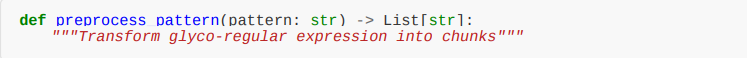
\includegraphics[scale=0.5]{Imagens/Figura 3_1.png}
  	\textsf{\caption{Implementação da função process\_pattern}}
  	\label{fig:implementação da função process\_pattern}
\end{figure}

\subsection{Exemplo de uso}

Considere a expressão regular de glicano $ex-HexNAc-([Hex|Fuc])\{1,2\}-HexNAc$. Esta expressão busca um padrão que começa com $Hex$, seguido por $HexNAc$, depois um ou dois $Hex$ ou $Fuc$, e termina com $HexNAc$.

\begin{figure}[H]
	\centering
  	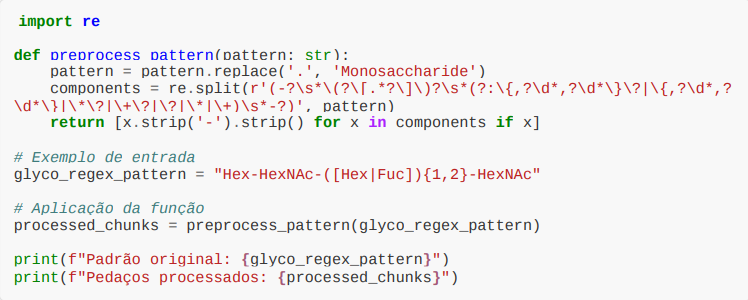
\includegraphics[scale=0.5]{Imagens/Figura 3_2.png}
  	\textsf{\caption{Aplicação da função process\_pattern}}
  	\label{fig:aplicação da função process\_pattern}
\end{figure}

\subsection{Comportamento de entrada}

Para a entrada $Hex-HexNAc-([Hex|Fuc])\{1,2\}-HexNAc$ , a função $preprocess\_pattern$ irá:
\begin{enumerate}
	\item Substituir qualquer $.$ por Monosaccharide;
	\item Dividir a string em componentes com base em um padrão de expressão regular que identifica modificadores e quantificadores $( [Hex|Fuc] , {1,2} )$;
	\item Remover strings vazias e espaços em branco, além de hífens ( - ) das extremidades dos componentes.
\end{enumerate}

O resultado esperado será uma lista de strings, onde cada string representa um "pedaço" da expressão regular de glicano, pronto para ser processado por outras funções do framework.

\section{specify\_linkages}

A função $specify\_linkages$ converte notações abreviadas de ligações em sua forma completa. Isso é essencial para padronizar as representações de glicanos e garantir que as operações de grafo possam interpretar corretamente as ligações entre os monossacarídeos.

\begin{figure}[htb]
	\centering
  	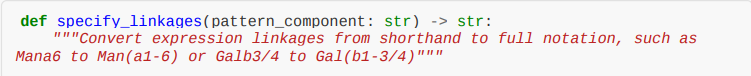
\includegraphics[scale=0.5]{Imagens/Figura 3_3.png}
  	\textsf{\caption{Implementação da função specify\_linkages}}
  	\label{fig:implementação da função specify\_linkages}
\end{figure}

\subsection{Exemplo de uso}

Considere um componente de padrão como $Mana6$ ou $Galb3/4$.

\begin{figure}[H]
	\centering
  	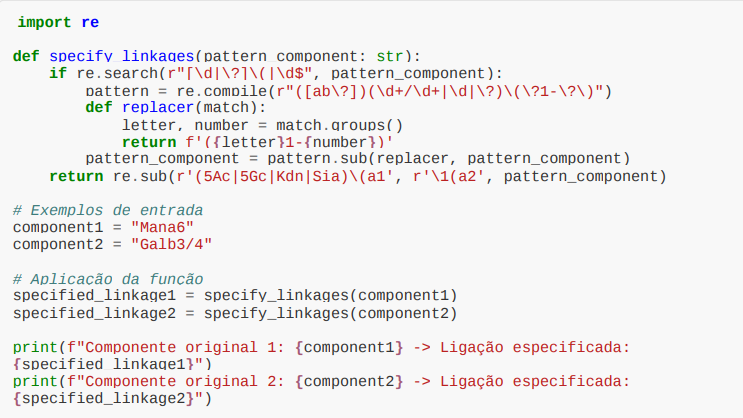
\includegraphics[scale=0.5]{Imagens/Figura 3_4.png}
  	\textsf{\caption{Aplicação da função specify\_linkages}}
  	\label{fig:aplicação da função specify\_linkages}
\end{figure}

\subsection{Comportamento de entrada}

Para $Mana6$, a função identificaria a notação abreviada e a converteria para $Man(a1-6)$. Similarmente, $Galb3/4$ seria convertida para $Gal(b1-3/4)$. Esta padronização é vital para a consistência na representação das ligações glicosídicas.

\section{get\_match}

A função $get_match$ é a principal interface para encontrar correspondências de uma expressão regular de glicano em uma estrutura de glicano. Ela utiliza as funções auxiliares como $preprocess_pattern$ e $specify\_linkages$ internamente para realizar a correspondência de padrões baseada em grafos.

\begin{figure}[htb]
	\centering
  	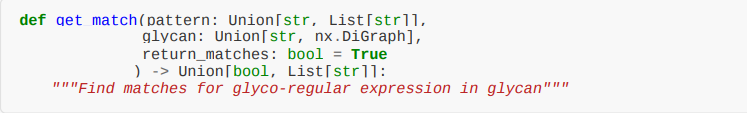
\includegraphics[scale=0.5]{Imagens/Figura 3_5.png}
  	\textsf{\caption{Implementação da função get\_match}}
  	\label{fig:implementação da função get\_match}
\end{figure}

\subsection{Exemplo de uso}

Para um exemplo prático de $get\_match$, precisaríamos de um ambiente glycowork completo, incluindo a capacidade de converter strings de glicanos em objetos networkx.DiGraph. No entanto, podemos ilustrar o conceito com um exemplo simplificado de como a função seria invocada e o tipo de resultado esperado.

\begin{figure}[H]
	\centering
  	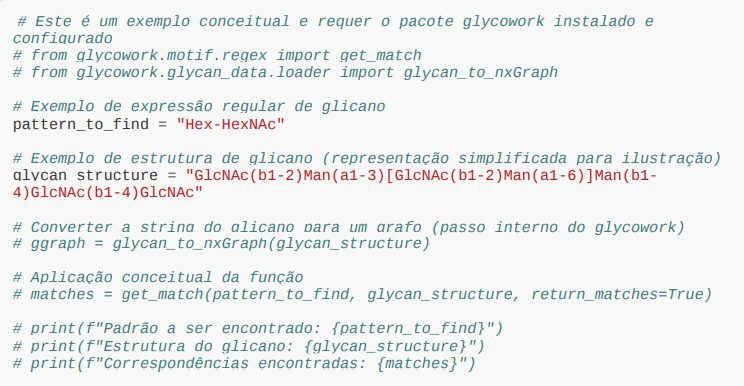
\includegraphics[scale=0.5]{Imagens/Figura 3_6.png}
  	\textsf{\caption{Aplicação da função specify\_linkages}}
  	\label{fig:aplicação da função specify\_linkages}
\end{figure}

\subsection{Comportamento de entrada}

Quando $get\_match$ é chamada com um pattern (expressão regular de glicano) e um glycan (estrutura de glicano), ela realiza os seguintes passos:

\begin{enumerate}
	\item Pré-processamento do Padrão: Utiliza $preprocess\_pattern$ para quebrar a expressão regular em componentes;
	\item Conversão do Glicano: Se o glicano for fornecido como string, ele é convertido para um objeto $networkx.DiGraph$, que é a representação interna usada para operações de grafo;
	\item Correspondência de Padrões Baseada em Grafo: A função então executa um algoritmo de correspondência de subgrafo para encontrar todas as ocorrências do padrão dentro do grafo do glicano;
	\item Formatação dos Resultados: Se $return\_matches$ for True, a função retorna uma lista de strings, onde cada string representa uma subestrutura de glicano que corresponde ao padrão. Caso contrário, retorna um booleano indicando se alguma correspondência foi encontrada.
\end{enumerate}

Este processo permite que o framework glycowork identifique padrões complexos em estruturas de glicanos, superando as limitações das expressões regulares textuais tradicionais ao considerar a topologia e as ligações químicas dos glicanos.